%\documentclass[handout]{mcs}

\begin{document}

\inclassproblems{6, Mon.}

%%%%%%%%%%%%%%%%%%%%%%%%%%%%%%%%%%%%%%%%%%%%%%%%%%%%%%%%%%%%%%%%%%%%%
% Problems start here
%%%%%%%%%%%%%%%%%%%%%%%%%%%%%%%%%%%%%%%%%%%%%%%%%%%%%%%%%%%%%%%%%%%%%

\begin{staffnotes}
Infinite Cardinality;  Ch. 8.1.1--8.1.3
\end{staffnotes}

\pinput{CP_countable_surjection-alt}

\pinput{CP_rationals_are_countable}
\hint Use Problem 1.

%\pinput{FP_uncountable_infinite_sequences}

\pinput{CP_smallest_infinite_set}

\pinput{PS_unit_interval}

\begin{center}
\textbf{Supplemental (Optional)}
\end{center}
\pinput{CP_Schroeder_Bernstein_theorem}  %more suited for pset




%%%%%%%%%%%%%%%%%%%%%%%%%%%%%%%%%%%%%%%%%%%%%%%%%%%%%%%%%%%%%%%%%%%%%
% Problems end here
%%%%%%%%%%%%%%%%%%%%%%%%%%%%%%%%%%%%%%%%%%%%%%%%%%%%%%%%%%%%%%%%%%%%%
\end{document}

%\input{cp6t}
%\input{cp6r}
%\documentclass[handout]{mcs}

\begin{document}

\inclassproblems{7, Mon.}

%%%%%%%%%%%%%%%%%%%%%%%%%%%%%%%%%%%%%%%%%%%%%%%%%%%%%%%%%%%%%%%%%%%%%
% Problems start here
%%%%%%%%%%%%%%%%%%%%%%%%%%%%%%%%%%%%%%%%%%%%%%%%%%%%%%%%%%%%%%%%%%%%%
%from S11 cp6w:

\pinput{CP_de_Bruijn_graphs}
\pinput{CP_covering_edges}
\pinput{CP_walk_relation_composition}


\iffalse
%\pinput{CP_directed_walks_and_cycles}
\pinput{CP_de_Bruijn_graphs}
\pinput{CP_tournament_chain}
%\pinput{CP_covering_edges}
\pinput{PS_walk_relation_composition}
\fi



%%%%%%%%%%%%%%%%%%%%%%%%%%%%%%%%%%%%%%%%%%%%%%%%%%%%%%%%%%%%%%%%%%%%%
% Problems end here
%%%%%%%%%%%%%%%%%%%%%%%%%%%%%%%%%%%%%%%%%%%%%%%%%%%%%%%%%%%%%%%%%%%%%
\end{document}



%\documentclass[handout]{mcs}

\begin{document}

\renewcommand{\reading}
{
  \emph{For this pset}:
  Sections~\bref{Turing_sec}{--}\bref{mod_prime_sec}{ on Modular Arithmetic}, and
  Sections~\bref{arithmetic_modn_sec}{ on Euler's Theorem}.
  %Section~\bref{state_machine_sec}{ on State Machines}, 
  %Chapter~\bref{recursive_data_chap}{ on Recursive Data}, and 
  %Sections~\bref{divisibility_sec}{--}
  %  ~\bref{fundamental_theorem_sec}{ on Number Theory.}

\emph{For lecture, Friday, Oct. 14}:
Sections~\bref{RSA_sec}{--}\bref{SAT_RSA-sec}{ on The RSA crypto-system}.
%Section~\bref{Turing_sec}{--}~\bref{mod_prime_sec}{ on Modular Arithmetic.}
}

\problemset{5}


\emph{Reminders}:
\begin{itemize}
\item The final deadline for Online Tutor Problems TP.6 and a
  \href{http://courses.csail.mit.edu/6.042/fall11/courseinfo#comments}{Piazza
    comment} on the reading is Thursday, Oct. 13, 10PM.
\iffalse
\item Problems should be submitted separately following the pset
  \href{http://courses.csail.mit.edu/6.042/fall11/submission}{submission
    instructions}, and each problem should have a \emph{collaboration
    statement} at the beginning, with the requisite information
  written in or attached using the
  \href{http://courses.csail.mit.edu/6.042/fall11/submission_template.pdf}{collaboration
    statement template}.
\fi

\end{itemize}


%TOPICS: state machines invariance, recursive data, GCD's

%%%%%%%%%%%%%%%%%%%%%%%%%%%%%%%%%%%%%%%%%%%%%%%%%%%%%%%%%%%%%%%%%%%%%
% Problems start here
%%%%%%%%%%%%%%%%%%%%%%%%%%%%%%%%%%%%%%%%%%%%%%%%%%%%%%%%%%%%%%%%%%

% PSET PROBLEMS FOR WEEK 5 FRIDAY
\pinput{PS_calculating_inverses} % I can change the numbers if necessary.

%\pinput{PS_self-inverse_mod_p} % Should remove all mention of the theorem name; move it to the solution
                               % so students don't just look up the proof.
%\pinput{CP_polynomials_produce_multiples} % New to repo; hints and restructuring may be in order.

% PSET PROBLEMS FOR WEEK 6 WEDNESDAY
%cp6w + mq7m: \pinput{PS_Euler_theorem_calculation}
%reject: \pinput{CP_13th_roots}
\pinput{FP_modular_powerful}
\pinput{PS_Euler_function_multiplicativity}

%mq7m: \pinput{TP_Relative_Primality}

% PSET PROBLEMS FOR WEEK 6 FRIDAY
%cp6f: \pinput{PS_RSA_correctness}
%reject: \pinput{PS_RSA_key_implies_factoring}
%reject: \pinput{PS_Rabin_cryptosystem}

% CLASS PROBLEMS FOR WEEK 6 WEDNESDAY
%\pinput{PS_Euler_theorem_calculation}
%\pinput{PS_congruent_modulo_1000}
%\pinput{CP_chinese_remainder}
%\pinput{PS_Euler_function_multiplicativity}

% CLASS PROBLEMS FOR WEEK 6 FRIDAY
%\pinput{CP_RSA_between_tables}
%\pinput{CP_RSA_proving_correctness}

% MINIQUIZ PROBLEMS: MORNING
%\pinput[points = 5]{MQ_Euler_function_of_100}
%\pinput[points = 5]{TP_Relative_Primality_6042}
%\pinput[points = 5]{FP_Euler_theorem_calculation}
%\pinput[points = 5]{TP_Eulers_Theorem}

% MINIQUIZ PROBLEMS: AFTERNOON
%\pinput[points = 5]{MQ_Euler_function_of_6042}
%\pinput[points = 5]{TP_Relative_Primality}

% COPIED FROM spring11/ps5.tex
%%\pinput{CP_conquering_the_galaxy}
%%\pinput{PS_directed_Euler_circuits}
%\pinput{CP_binary_relations_on_01}
%\pinput{PS_top_sort_for_closure_of_DAG}
%\pinput{PS_Brents_theorem}
%%\pinput{CP_product_relation_properties}
%\pinput{PS_subsequences_partial_order_Dilworth_Lemma}
%%\pinput{PS_weak_partial_order_isomorphic_to_subset}

% COPIED FROM fall11/ps4.tex
%\pinput{CP_robot_invariant}
%\pinput{PS_bracket_good_count}
%\iffalse
%%NOT THIS WEEK
%\pinput{PS_calculating_inverses}
%\large\textbf{Repo: PS\_congruent\_modulo\_1000}
%\pinput{PS_congruent_modulo_1000}
%\large\textbf{Repo: PS\_RSA\_correctness}
%\pinput{PS_RSA_correctness}
%\fi
%%\large\textbf{Repo: CP\_binary\_trees}
%%\pinput{CP_binary_trees}
%\pinput{PS_linear_combination_by_structural_induction}
%\pinput{PS_labeled_binary_trees}
%%\large\textbf{Repo: PS\_linear\_combination\_game}
%%\pinput{PS_linear_combination_game}

%%%%%%%%%%%%%%%%%%%%%%%%%%%%%%%%%%%%%%%%%%%%%%%%%%%%%%%%%%%%%%%%%%%%%
% Problems end here
%%%%%%%%%%%%%%%%%%%%%%%%%%%%%%%%%%%%%%%%%%%%%%%%%%%%%%%%%%%%%%%%%%%%%
\end{document}


\chapter{Simple Graphs}
%\coursecopyright

%% Introduction %%%%%%%%%%%%%%%%%%%%%%%%%%%%%%%%%%%%%%%%%%%%%%%%%%%%%%%%%%%%%%%
Graphs arise in different fields with all sorts of applications,
including scheduling, optimization, communications, and the design and
analysis of algorithms.  Two Stanford students even used graph theory to
become multibillionaires!

But we'll start with an application designed to get your attention: we are
going to make a professional inquiry into sexual behavior.  Namely, we'll
look at some data about who, on average, who has more opposite-gender
partners, men or women?

Sexual demographics have been the subject of many studies.  In one of the
largest, researchers from the University of Chicago interviewed a random
sample of 2500 people over several years to try to get an answer to this
question.  Their study, published in 1994, and entitled \emph{The Social
  Organization of Sexuality} found that on average men have 74\% more
opposite-gender partners than women.

Other studies have found that the disparity is even larger.  In
particular, ABC News claimed that the average man has 20 partners over his
lifetime, and the average woman has 6, for a percentage disparity of
233\%.  The ABC News study, aired on Primetime Live in 2004, purported to
be one of the most scientific ever done, with only a 2.5\% margin of
error.  It was called "American Sex Survey: A peak between the sheets,"
---which makes its science start to sound a little doubtful.  \iffalse The
promotion for the study is even better:
\begin{quote} 
A ground breaking ABC News ``Primetime Live'' survey finds a range of
eye-popping sexual activities, fantasies and attitudes in this country,
confirming some conventional wisdom, exploding some myths -- and venturing
where few scientific surveys have gone before.
\end{quote}
Probably that last part about going where few scientific surveys have gone
before is pretty accurate!
\fi
Yet again, in August, 2007, the N.Y. Times
\href{http://www.nytimes.com/2007/08/12/weekinreview/12kolata.html?_r=1&n=Top/Reference/Times%20Topics/People/K/Kolata,%20Gina&oref=slogin}{reported} on a study by the
  National Center for Health Statistics of the U.S. government showing
  that men had seven partners while women had four.

  Anyway, whose numbers do you think are more accurate, the University of
  Chicago, ABC News, or the National Center?  Don't answer: this is a setup
  question like ``When did you stop beating your wife?''  Using a little
  graph theory, we'll explain why none of these findings can be anywhere
  near the truth.


%% Simple Graphs %%%%%%%%%%%%%%%%%%%%%%%%%%%%%%%%%%%%%%%%%%%%%%%%%%%%%%%%%%%%%%
\hyperdef{simple}{graphs}{\section{Simple Graphs}}

\subsection{Definition of Simple Graph}

Informally, a graph is a bunch of dots with lines connecting some of
them.  Here is an example:

\mfigure{!}{1.5in}{figures/graph-example.pdf}

For many Mathematical purposes, we don't really care how the points and
lines are laid out ---only which points are connected by lines.  The
definition of \emph{simple graphs} aims to capture just this connection
data.

\begin{definition}\label{graphdef} 
A \emph{simple graph}, $G$, consists of a nonempty set, $V$, called the
\emph{vertices} of $G$, and a collection, $E$, of two-element subsets of
$V$.  The members of $E$ are called the \emph{edges} of $G$.
\end{definition}

The vertices correspond to the dots in the picture, and the edges
correspond to the lines.  For example, the connection data in
dots-and-lines diagram above is a captured by the following simple graph:
\begin{eqnarray*}
V & = & \set{A, B, C, D, E, F, G, H, I} \\
E & = & \set{ \set{A, B}, \set{A, C}, \set{B, D}, \set{C, D},
              \set{C, E}, \set{E, F}, \set{E, G}, \set{H, I} }.
\end{eqnarray*}

It will be helpful to use the notation $\edge{A}{B}$ for the edge
$\set{A,B}$.  Note that $\edge{A}{B}$ and $\edge{B}{A}$ are different
descriptions of the same edge, since sets are unordered.

Two vertices in a simple graph are said to be \term{adjacent} if they are
joined by an edge, and an edge is said to be \term{incident} to the
vertices it joins.  The number of edges incident to a vertex is called the
\term{degree} of the vertex; equivalently, the degree of a vertex is
equals the number of vertices adjacent to it.  For example, in the simple
graph above, $A$ is adjacent to $B$ and $B$ is adjacent to $D$, and the
edge $\edge{A}{C}$ is incident to vertices $A$ and $C$.  Vertex $H$ has
degree 1, $D$ has degree 2, and $E$ has degree 3.

\subsubsection{Graph Synonyms}

A synonym for ``vertices'' is "nodes,'' and we'll use these words
interchangeably.

Simple graphs are sometimes called \emph{networks}, edges are sometimes
called \emph{arcs}, and adjacent vertices are sometimes called
\emph{neighbors}.  We mention this as a ``heads up'' in case you look at
other graph theory literature; we won't use these words.

Some technical consequences of Definition~\ref{graphdef} are worth noting
right from the start:
\begin{enumerate}
\item Simple graphs do not have edges going from a vertex
back around to itself (called a \emph{self-loop}).

\item There is at most one edge between two vertices of a simple graph.

\item Simple graphs have at least one vertex, though they might not have
any edges.
\end{enumerate}
There's no harm in relaxing these conditions, and some authors do, but we
don't need self-loops, multiple edges between the same two vertices, or
graphs with no vertices, and it's simpler not to have them around.

For the rest of these Notes we'll only be considering simple graphs, so
we'll just call them ``graphs'' from now on.

\hyperdef{sex}{america}{\subsection{Sex in America}\label{sexam}}

%A 1994 University of Chicago study entitled \textit{The Social
%Organization of Sexuality} found that on average men have 74\% more
%opposite-gender partners than women.

Let's model the question of heterosexual partners in graph theoretic
terms.  To do this, we'll let $G$ be the graph whose vertices, $V$, are
all the people in America.  Then we split $V$ into two separate subsets:
$M$, which contains all the males, and $F$, which contains all the
females.\footnote{For simplicity, we'll ignore the possibility of someone
  being both, or neither, a man and a woman.}  We'll put an edge between a
male and a female iff they have been sexual partners.  This graph is
pictured in Figure~\ref{fig:partners} with males on the left and females on
the right.

\begin{figure}[htbp]
\centering 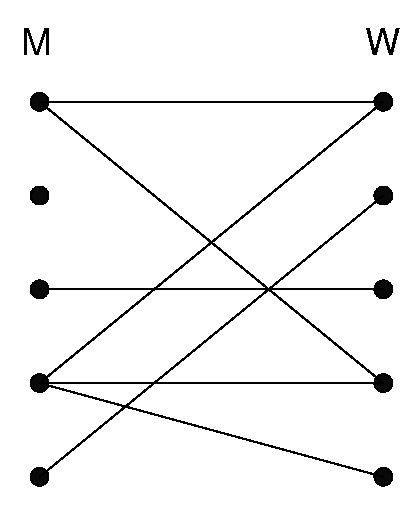
\includegraphics[height=1.75in]{figures/sex-edges.pdf}
\caption{The sex partners graph}
\label{fig:partners}
\end{figure}

Actually, this is a pretty hard graph to figure out, let alone draw.  The
graph is \emph{enormous}: the US population is about 300 million, so
$\card{V} \approx 300M$!  Of these, approximately 50.8\% are female and
49.2\% are male, so $\card{M} \approx 147.6M$, and $\card{F} \approx
152.4M$.  And we don't even have trustworthy estimates of how many edges
there are, let alone exactly which couples are adjacent.

But it turns out that we don't need to know any of this ---we just need to
figure out the relationship between the average number of partners per
male and partners per female.  To do this, we note that every edge is
incident to exactly one $M$ vertex (remember, we're only considering
male-female relationships); so the sum of the degrees of the $M$ vertices
equals the number of edges.  For the same reason, the sum of the degrees
of the $F$ vertices equals the number of edges.  So these sums are equal:
%
\[
\sum_{x \in M} \degr{x} = \sum_{y \in F} \degr{y}.
\]
%
Now suppose we divide both sides of this equation by the product of
the sizes of the two sets, $\card{M} \cdot \card{F}$:
%
\[
\left(\frac{\sum_{x \in M} \degr{x}}{\card{M}}\right) \cdot \frac{1}{\card{F}} =
\left(\frac{\sum_{y \in F} \degr{y}}{\card{F}}\right) \cdot \frac{1}{\card{M}}
\]
%
The terms above in parentheses are the \textit{average degree of an $M$
vertex} and the \textit{average degree of a $F$} vertex.  So we know:
\[
\text{Avg. deg in $M$} = \frac{\card{F}}{\card{M}} \cdot \text{Avg. deg in $F$}
\]

In other words, we've proved that the average number of female partners of
males in the population compared to the average number of males per
female is \emph{determined solely by the relative number of males and
females in the population}.

Now the Census Bureau reports that there are slightly more females than
males in America; in particular $\card{F} / \card{M}$ is about 1.035.  So
we know that on average, males have 3.5\% more opposite-gender partners
than females, and this tells us nothing about any sex's promiscuity or
selectivity.  Rather, it just has to do with the relative number of males
and females.  Collectively, males and females have the same number of
opposite gender partners, since it takes one of each set for every
partnership, but there are fewer males, so they have a higher ratio.  So the
University of Chicago, ABC, and the Federal government studies are way
off.  After a huge effort, they gave a totally wrong answer.

There's no definite explanation for why such surveys are consistently
wrong.  One hypothesis is that males exaggerate their number of partners
---or maybe females downplay theirs ---but these explanations are
speculative.  Interestingly, the principal author of the National Center
for Health Statistics study reported that she knew the results had to be
wrong, but that was the data collected and her job was to report that.

The same underlying issue has led to serious misinterpretations of other
survey data.  For example, a couple of years ago, the Boston Globe ran a
story on a survey of the study habits of students on Boston area campuses.
Their survey showed that on average, minority students tended to study
with non-minority students more than the other way around.  They went on
at great length to explain why this ``remarkable phenomenon'' might be
true.  But it's not remarkable at all ---using our graph theory
formulation, we can see that all it says is that there are fewer minority
students than non-minority students.  Well, that just follows from the
definition of ``minority''!

\subsection{Handshaking Lemma}

The previous argument hinged on the connection between a sum of degrees
and the number edges.  There is a simple connection between these in any
graph:

\begin{theorem}\label{sumedges}
The sum of the degrees of the vertices in a graph equals twice the number
of edges.
\end{theorem}

\begin{proof}
Every edge contributes two to the sum of the degrees, one for each of its
endpoints.
\end{proof}

Theorem~\ref{sumedges} is sometimes called the \emph{Handshake Theorem}:
if we total up the number of people each person at a party shakes hands
with, the total will be twice the number of handshakes that occurred.

\subsection{Some Common Graphs}

Some graphs come up so frequently that they have names.  The {\em complete
graph} on $n$ vertices, also called $K_n$, has an edge between every two
vertices.  Here is $K_5$:

\mfigure{!}{1.5in}{figures/complete-graph.pdf}

The {\em empty graph} has no edges at all.  Here is the
empty graph on 5 vertices:

\mfigure{!}{1.5in}{figures/empty-graph.pdf}

Another 5 vertex graph is $L_4$, the \emph{line graph} of length four:

\mfigure{!}{1in}{figures/path-graph.pdf}

And here is $C_5$, a \emph{simple cycle} with 5 vertices:

\mfigure{!}{1.5in}{figures/cycle.pdf}

\subsection{Isomorphism}

Two graphs that look the same might actually be different in a formal
sense.  For example, the two graphs below are both simple cycles with
4~vertices:

\mfigure{!}{1.5in}{figures/isomorphism.pdf}

But one graph has vertex set $\set{A, B, C, D}$ while the
other has vertex set $\set{1, 2, 3, 4}$.  If so, then the graphs are
different mathematical objects, strictly speaking.  But this is a
frustrating distinction; the graphs {\em look the same}!

Fortunately, we can neatly capture the idea of ``looks the same.''  Graphs
$G_1$ and $G_2$ are {\em isomorphic} if there exists a bijection between
the vertices in $G_1$ and the vertices in $G_2$ such that there is an edge
between two vertices in $G_1$ if and only if there is an edge between the
two corresponding vertices in $G_2$.  For example, take the following
bijection between vertices in the two graphs above:
\[
\begin{array}{lll}
A \text{ corresponds to } 1 & \hspace{0.5in} & B \text{ corresponds to } 2 \\
D \text{ corresponds to } 4 & & C \text{ corresponds to } 3.
\end{array}
\]
Now there is an edge between two vertices in the graph on the left if and
only if there is an edge between the two corresponding vertices in the
graph on the right.  Therefore, the two graphs are isomorphic.  The
bijection itself is called an {\em isomorphism}.
\begin{definition}
If $G_1$ is a graph with vertices, $V_1$, and edges,
$E_1$, and likewise for $G_2$, then $G_1$ is {\em isomorphic} to $G_2$ iff
there exists a \textbf{bijection}, $f: V_1 \to V_2$, such that for
every pair of vertices $u, v \in V_1$:
\[
\edge{u}{v} \in E_1 \qiff \edge{f(u)}{f(v)} \in E_2.
\]
The function $f$ is called an {\em isomorphism} between $G_1$ and
$G_2$.
\end{definition}

Two isomorphic graphs may be drawn very differently.  For example, here
are two different ways of drawing $C_5$:

\mfigure{!}{1.5in}{figures/isomorphism-c5.pdf}

Isomorphism captures all the connection properties of a graph, abstracting
out what the vertices are called, what they are made out of, or where they
appear in a drawing of the graph.  So a property like ``having three
vertices of degree 4'' is preserved under isomorphism, while ``having a
vertex that is an integer'' is not preserved.  In particular, if one graph
has three vertices of degree 4 and another does not, they can't be
isomorphic.  Similarly, if one graph has an edge that is incident to
a degree 8 vertex and a degree 3 vertex, then any isomorphic graph must also
have such an edge.

Looking for properties like these can make it easy to determine that two
graphs are not isomorphic, or to actually find an isomorphism between
them, if there is one.  In practice, it's frequently easy to decide
whether two graphs are isomorphic.  However, no one has yet found a
\emph{general} procedure for determining whether two graphs are isomorphic
which is \emph{guaranteed} to run much faster than an exhaustive (and
exhausting) search through all possible bijections between their
vertices.

Having an efficient procedure to detect isomorphic graphs would, for
example, make it easy to search for a particular molecule in a database
given the molecular bonds.  On the other hand, knowing there is no such
efficient procedure would also be valuable: secure protocols for
encryption and remote authentication can be built on the hypothesis that
graph isomorphism is computationally exhausting.

%% Simple Graphs Problems %%%%%%%%%%%%%%%%%%%%%%%%%%%%%%%%%%%%%%%%%%%%%%%%%%%%%
%\startclassproblems
%\pinput{CP_handshaking_proofs}
%\pinput{CP_isomorphism_finger_exercise}
%\pinput{CP_neighbors_under_isomorphism}
% S09.cp6m.1
% S09.cp6m.3
% S09.cp6m.4


%% Connectedness %%%%%%%%%%%%%%%%%%%%%%%%%%%%%%%%%%%%%%%%%%%%%%%%%%%%%%%%%%%%%%
\hyperdef{connect}{edness}{\section{Connectedness}}

\subsection{Paths and Simple Cycles}

A \emph{path} in a graph describes how to get from one vertex to another
following edges of the graph.  Formally,

\begin{definition}
A \term{path} in a graph, $G$, is a sequence of $k \geq 0$ vertices
\[
v_0,\dots,v_k
\]
such that $\edge{v_i}{v_{i+1}}$ is an edge of $G$ for all $i$ where $0
\leq i < k$ .  The path is said to \term{start} at $v_0$, to \term{end} at
$v_k$, and \term{length} of the path is defined to be $k$.  An edge,
$\edge{u}{v}$, is \term{traversed $n$ times} by the path if there are $n$
different values of $i$ such that $\edge{v_i}{v_{i+1}} = \edge{u}{v}$.

The path is \term{simple}\footnote{Heads up if you read another graph
  theory text: what amounts to paths are commonly referred to as
  ``walks,'' and simple paths are referred to as a just ``paths''.
  Likewise, what we will call \emph{cycles} and \emph{simple cycles}
  are commonly called ``closed walks'' and just ``cycles''.}  iff all
the $v_i$'s are different, that is, $v_i = v_j$ only if $i=j$.

\end{definition}

For example, the graph in Figure~\ref{dg} has a length~6 simple path
A,B,C,D,E,F,G.  This is the longest simple path in the graph.

\begin{figure}[htbp] 
\mfigure{!}{1.75in}{figures/distance-graph.pdf}
\caption{\em A graph with 3 simple cycles.}
\label{dg}
\end{figure}

Notice that the {\em length} of a path is the total number of times it
traverses edges, which is \emph{one less} than its length as a sequence of
vertices.  The length~6 path A,B,C,D,E,F,G is actually a sequence of seven
vertices.

A \emph{cycle} can be described by a path \iffalse of length two or
more\fi that begins and ends with the same vertex.  For example,
B,C,D,E,C,B is a cycle in the graph in Figure~\ref{dg}.  This path
suggests that the cycle begins and ends at vertex B, but a cycle isn't
intended to have a beginning and end, and can be described by \emph{any}
of the paths that go around it.  For example, D,E,C,B,C,D describes this
same cycle as though it started and ended at D, and D,C,B,C,E,D describes
the same cycle as though it started and ended at D but went in the
opposite direction.  (By convention, a single vertex is a length 0 cycle
beginning and ending at the vertex.)

All the paths that describe the same cycle have the same length which is
defined to be the {\em length} of the cycle.  (Note that this implies that
going around the same cycle twice is considered to be different than going
around it once.)

A \emph{simple} cycle is a cycle that doesn't cross or backtrack on
itself.  For example, the graph in Figure~\ref{dg} has three simple cycles
B,H,E,C,B and C,D,E,C and B,C,D,E,H,B.  More precisely, a simple cycle is
a cycle that can be described by a path of length at least three whose
vertices are all different except for the beginning and end vertices.  So
in contrast to simple \emph{paths}, the length of a simple \emph{cycle} is
the \emph{same} as the number of distinct vertices that appear in it.

From now on we'll stop being picky about distinguishing a cycle from a
path that describes it, and we'll just refer to the path as a cycle.
\footnote{Technically speaking, we haven't ever defined what a cycle
\emph{is}, only how to describe it with paths.  But we won't need an
abstract definition of cycle, since all that matters about a cycle is which
paths describe it.}

\iffalse

Simple cycles are especially important, so we will give a proper
definition of them.  Namely, we'll define a simple cycle in $G$ to be a
\emph{subgraph} of $G$ that looks like a cycle that doesn't cross itself.
Formally:

\begin{definition}
A \term{subgraph}, $G'$, of a graph, $G$, is a graph whose vertices, $V'$,
are a subset of the vertices of $G$ and whose edges are a subset
of the edges of $G$.
\end{definition}
Notice that since a subgraph is itself a graph, the endpoints of every
edge of $G'$ must be vertices in $V'$.

\begin{definition}
For $n \ge 3$, let $C_n$ be the graph with vertices $1,\dots, n$ and
edges
\[
\edge{1}{2},\ \ \edge{2}{3},\ \ \dots,\ \ \edge{(n-1)}{n},\ \ \edge{n}{1}.
\]
 graph is a \term{simple cycle of length $n$} iff it is isomorphic to
$C_n$ for some $n \ge 3$.  A \term{simple cycle of a graph}, $G$, is a
subgraph of $G$ that is a simple cycle.
\end{definition}
\fi


\subsection{Connected Components}

\begin{definition}
Two vertices in a graph are said to be \term{connected} if there is a path
that begins at one and ends at the other.
\end{definition}

By convention, every vertex is considered to be connected to itself by a
path of length zero.

\iffalse

Now if there is a path from vertex $u$ to vertex $v$, then $v$ is
connected to $u$ by the reverse path, so connectedness is a symmetric
relation.  Also, if there is a path from $u$ to $v$, and also a path from
$v$ to $w$, then these two paths can be combined to form a path from $u$
to $w$.  So the connectedness relation is transitive.  It is also
reflexive, since every vertex is by definition connected to itself by a
path of length zero.
\fi

The diagram in Figure~\ref{fig:3comp} looks like a picture of three
graphs, but is intended to be a picture of \emph{one} graph.  This graph
consists of three pieces (subgraphs).  Each piece by itself is connected,
but there are no paths between vertices in different pieces.

\iffalse
\begin{figure}[htbp]
\mfigure{!}{1.5in}{figures/3comp.pdf}
% \centerline{\psfig{figure=figures/3comp.eps,height=1.5in}}
\caption{\em One graph with 3 connected components.}
\label{fig:3comp}
\end{figure}
\fi

\begin{figure}[htbp] 
\mfigure{!}{1.5in}{figures/connectivity-graphs.pdf}
\caption{\em One graph with 3 connected components.}
\label{fig:3comp}
\end{figure}

\begin{definition}
A graph is said to be \term{connected} if every pair of vertices are
connected.
\end{definition}

These connected pieces of a graph are called its \term{connected
components}.  A rigorous definition is easy: a connected component is the
set of all the vertices connected to some single vertex.  So a graph is
connected iff it has exactly one connected component.  The empty graph on
$n$ vertices has $n$ connected components.

\subsection{How Well Connected?}

If we think of a graph as modelling cables in a telephone network, or oil
pipelines, or electrical power lines, then we not only want connectivity,
but we want connectivity that survives component failure.  A graph is
called \emph{$k$-edge connected} if it remains connected as long as fewer
than $k$ ``direct connections between components fail,'' that is, it stays
connected even if as many as $k-1$ edges are deleted.  More precisely:
\begin{definition}
  Two vertices in a graph are \term{$k$-edge connected} if they remain
  connected in every subgraph obtained by deleting $k-1$ edges.  A graph
  with at least two vertices is $k$-edge connected\footnote{The
    corresponding definition of connectedness based on deleting vertices
    rather than edges is common in Graph Theory texts and is usually
    simply called ``$k$-connected'' rather than ``$k$-vertex connected.''}
  if every two of its vertices are $k$-edge connected.
\end{definition}
So 1-edge connected is the same as connected for both vertices and graphs.
Another way to say that a graph is $k$-edge connected is that every
subgraph obtained from it by deleting at most $k-1$ edges is connected.

For example, in the graph in Figure~\ref{dg}, vertices B and E are
2-edge connected, G and E are 1-edge connected, and no vertices are 3-edge connected.
The graph as a whole is only 1-edge connected.

More generally, any simple cycle is 2-edge connected, and the complete graph,
$K_n$, is $(n-1)$-edge connected.

If two vertices are connected by $k$ edge-disjoint paths (that is, no two
paths traverse the same edge), then they are obviously $k$-edge connected.
A fundamental fact, whose ingenious proof we omit, is Menger's theorem
which confirms that the converse is also true: if two vertices are
$k$-edge connected, then there are $k$ edge-disjoint paths connecting
them.  It takes some ingenuity to prove this even for the case $k=2$.




\subsection{Connection by Simple Path}

Where there's a path, there's a simple path.  This is sort of obvious, but
it's easy enough to prove rigorously using the Well-ordering Principle.

\begin{lemma}\label{simplepath}
If vertex $u$ is connected to vertex $v$ in a graph, then there is a
simple path from $u$ to $v$.
\end{lemma}

\begin{proof}
Since there is a path from $u$ to $v$, there must, by the Well-ordering
Principle, be a minimum length path from $u$ to $v$.  If the minimum
length is zero or one, this minimum length path is itself a simple path
from $u$ to $v$.

Otherwise, there is a minimum length path
\[
v_0, v_1,\dots, v_k
\]
from $u = v_0$ to $v = v_k$ where $k \geq 2$.  We claim this path must be
simple.

To prove the claim, suppose to the contrary that the path is not simple,
that is, some vertex on the path occurs twice.  This means that there are
integers $i,j$ such that $0 \leq i < j \leq k$ with $v_i= v_j$.  Then
deleting the subsequence
\[
v_{i+1}, \dots v_j
\]
yields a strictly shorter path
\[
v_0, v_1,\dots, v_i,v_{j+1},v_{j+2},\dots, v_k
\]
from $u$ to $v$, contradicting the minimality of the given path.
\end{proof}

Actually, we proved something stronger:
\begin{corollary}\label{ss}
For any path of length $k$ in a graph, there is a simple path of length
\emph{at most} $k$ with the same endpoints.
\end{corollary}

\subsection{The Minimum Number of Edges in a Connected Graph}

The following theorem says that a graph with few edges must have many
connected components.

\begin{theorem} \label{th:connectivity}
Every graph with $v$ vertices and $e$ edges has at least $v - e$ connected
components.
\end{theorem}

Of course for Theorem~\ref{th:connectivity} to be of any use, there must
be fewer edges than vertices.

\begin{proof}
We use induction on the number of edges, $e$.  Let $P(e)$ be the
proposition that
\begin{quote}
for every $v$, every graph with $v$ vertices and $e$ edges has at least
$v-e$ connected components.
\end{quote}

\textbf{Base case:}($e=0$).  In a graph with 0 edges and $v$ vertices,
each vertex is itself a connected component, and so there are exactly $v =
v - 0$ connected components.  So $P(e)$ holds.

\textbf{Inductive step:} Now we assume that the induction hypothesis holds
for every $e$-edge graph in order to prove that it holds for every
$(e+1)$-edge graph, where $e \geq 0$.

Consider a graph, $G$, with $e + 1$ edges and $k$ vertices.  We want to
prove that $G$ has at least $v - (e+1)$ connected components.

To do this, remove an arbitrary edge $\edge{a}{b}$ and call the resulting
graph $G'$.  By the induction assumption, $G'$ has at least $v - e$
connected components.

Now add back the edge $\edge{a}{b}$ to obtain the original graph $G$.  If
$a$ and $b$ were in the same connected component of $G'$, then $G$ has the
same connected components as $G'$, so $G$ has at least $v -e > v - (e+1)$
components.  Otherwise, if $a$ and $b$ were in different connected
components of $G'$, then these two components are merged into one in $G$,
but all other components remain unchanged, reducing the number of
components by 1.  Therefore, $G$ has at least $(v - e) - 1 = v - (e+1)$
connected components.  So in either case, $P(e+1)$ holds.  This completes
the Induction step.

The theorem now follows by induction.
\end{proof}

\begin{corollary}
\label{cor:n-1}
Every connected graph with $v$ vertices has at least $v - 1$ edges.
\end{corollary}

A couple of points about the proof of Theorem~\ref{th:connectivity} are
worth noting.  First, notice that we used induction on the number of edges
in the graph.  This is very common in proofs involving graphs, and so is
induction on the number of vertices.  When you're presented with a graph
problem, these two approaches should be among the first you consider.

The second point is more subtle.  Notice that in the inductive step, we
took an arbitrary $(n+1)$-edge graph, threw out an edge so that we could
apply the induction assumption, and then put the edge back.  You'll see
this shrink-down, grow-back process very often in the inductive steps of
proofs related to graphs.  This might seem like needless effort; why not
start with an $n$-edge graph and add one more to get an $(n+1)$-edge
graph?  That would work fine in this case, but opens the door to a nasty
logical error called \emph{buildup} error, illustrated in
Problem~\ref{buildup}.\ below.
\iffalse You'll see an example in class.\fi
Always use shrink-down, grow-back arguments, and you'll never
fall into this trap.

%S08, cp6m, S06 cp5f

%S06 cp5f


\begin{notesproblem}\label{buildup}
\bparts

\ppart Give a counterexample to the
\begin{falseclm*}
If every vertex in a graph has positive degree, then the graph is
connected.
\end{falseclm*}

\begin{solution}
There are many counterexamples; here is one:

\mfigure{!}{0.75in}{figures/false-connect-cx.pdf}

\end{solution}

\ppart Since the Claim is false, there must be an logical mistake in the
following bogus proof of it.  Pinpoint the first logical mistake
(unjustified step) in this proof.

\begin{bogusproof}
  We prove the Claim above by induction.  Let $P(n)$ be the proposition
  that if every vertex in an $n$-vertex graph has positive degree, then
  the graph is connected.

\textbf{Base cases}: ($n \leq 2$).  In a graph with 1 vertex, that vertex
cannot have positive degree, so $P(1)$ holds vacuously.

$P(2)$ holds because there is only one graph with two vertices of positive
degree, namely, the graph with an edge between the vertices, and this
graph is connected.

\textbf{Inductive step}: We must show that $P(n)$ implies
$P(n+1)$ for all $n \geq 2$.  Consider an $n$-vertex graph in which every
vertex has positive degree.  By the assumption $P(n)$, this graph is
connected; that is, there is a path between every pair of vertices.  Now
we add one more vertex $x$ to obtain an $(n+1)$-vertex graph:

\mfigure{!}{1.75in}{figures/false-connect-pic.pdf}

All that remains is to check that there is a path from $x$ to every other
vertex $z$.  Since $x$ has positive degree, there is an edge from $x$ to
some other vertex; call it $y$.  Thus, we can obtain a path from $x$ to
$z$ by adjoining the edge $\edge{x}{y}$ to the path from $y$ to $z$.  This
proves $P(n+1)$.

By the principle of induction $P(n)$ is true for all $n \geq 0$, which
proves the Claim.

\end{bogusproof}

\begin{solution}
This one is tricky: the proof is actually a good proof of
something else.  The first error in the proof is only in the final
statement of the inductive step: ``This proves $P(n+1)$''.

The issue is that to prove $P(n+1)$, \emph{every} $(n+1)$-vertex
positive-degree graph must be shown to be connected.  But the proof
doesn't show this.  Instead, it shows that every $(n+1)$-vertex
positive-degree graph \emph{that can be built up by adding a vertex of
positive degree to an $n$-vertex connected graph}, is connected.

The problem is that \emph{not every} $(n+1)$-vertex positive-degree graph
can be built up in this way.  The counterexample above illustrates this:
there is no way to build that 4-vertex positive-degree graph from a
3-vertex positive-degree graph.

More generally, this is an example of ``buildup error''.  This error
arises from a faulty assumption that every size $n+1$ graph with some
property can be ``built up'' in some particular way from a size $n$ graph
with the same property.  (This assumption is correct for some properties,
but incorrect for others--- such as the one in the argument above.)

One way to avoid an accidental build-up error is to use a ``shrink
down, grow back'' process in the inductive step: start with a size
$n+1$ graph, remove a vertex (or edge), apply the inductive hypothesis
$P(n)$ to the smaller graph, and then add back the vertex (or edge)
and argue that $P(n+1)$ holds.  Let's see what would have happened if
we'd tried to prove the claim above by this method:

\noindent \textit{Inductive step:} We must show that $P(n)$ implies
$P(n+1)$ for all $n \geq 1$.  Consider an $(n+1)$-vertex graph $G$ in
which every vertex has degree at least 1.  Remove an arbitrary vertex
$v$, leaving an $n$-vertex graph $G'$ in which every vertex has
degree... uh-oh!

The reduced graph $G'$ might contain a vertex of degree 0, making the
inductive hypothesis $P(n)$ inapplicable!  We are stuck--- and
properly so, since the claim is false!
\end{solution}

\eparts
\end{notesproblem}

%% Connectedness Problems %%%%%%%%%%%%%%%%%%%%%%%%%%%%%%%%%%%%%%%%%%%%%%%%%%%%%
%\startclassproblems
%\pinput{CP_}
% S09.cp6m.2
% S09.cp6t.1


%% Trees %%%%%%%%%%%%%%%%%%%%%%%%%%%%%%%%%%%%%%%%%%%%%%%%%%%%%%%%%%%%%%%%%%%%%%
%Used to come after Coloring: proof read for switched references
\section{Trees}

Trees are a fundamental data structure in Computer Science, and there are
many kinds, for example rooted, ordered, or binary trees.  In this section
we focus on the purest kind of tree.  Namely, we use the \term{tree} to
mean a connected graph without simple cycles.

A graph with no simple cycles is called \term{acyclic}; so trees are
acyclic connected graphs.

\subsection{Tree Properties}
Here is an example of a tree:

\mfigure{!}{1.5in}{figures/tree-example.pdf}

A vertex of degree at most one is called a \term{leaf}.  Note that the only
case where a tree can have a vertex of degree zero is a graph with a single
vertex.  In this example, there are 5~leaves.

The graph shown above would no longer be a tree if any edge were removed,
because it would no longer be connected.  The graph would also not remain
a tree if any edge were added between two of its vertices, because then it
would contain a simple cycle.  Furthermore, note that there is a unique
path between every pair of vertices.  These features of the example tree
are actually common to all trees.

\begin{theorem}
Every tree has the following properties:
\begin{enumerate}
\item Any connected subgraph is a tree.
\item There is a unique simple path between every pair of vertices.
\item Adding an edge between two vertices creates a cycle.
\item Removing any edge disconnects the graph.
\item If it has at least two vertices, then it has at least two leaves.
\item The number of vertices is one larger than the number of edges.
\end{enumerate}
\end{theorem}

\begin{proof}

\begin{enumerate}
\item\label{asub} A simple cycle in a subgraph is also a simple cycle in
the whole graph, so any subgraph of an acyclic graph must also be acyclic.
If the subgraph is also connected, then by definition, it is a tree.

\item There is at least one path, and hence one simple path, between every
pair of vertices, because the graph is connected.  Suppose that there are
two different simple paths between vertices $u$ and $v$.  Beginning at
$u$, let $x$ be the first vertex where the paths diverge, and let $y$ be
the next vertex they share.  Then there are two simple paths from $x$ to
$y$ with no common edges, which defines a simple cycle.  This is a
contradiction, since trees are acyclic.  Therefore, there is exactly one
simple path between every pair of vertices.

\mfigure{!}{1in}{figures/unique-path.pdf}

\item An additional edge $\edge{u}{v}$ together with the unique path
between $u$ and $v$ forms a simple cycle.

\item Suppose that we remove edge $\edge{u}{v}$.  Since a tree
contained a unique path between $u$ and $v$, that path must have been
$\edge{u}{v}$.  Therefore, when that edge is removed, no path remains,
and so the graph is not connected.

\item Let $v_1, \dots, v_m$ be the sequence of vertices on a longest
simple path in the tree.  Then $m \geq 2$, since a tree with two vertices
must contain at least one edge.  There cannot be an edge $\edge{v_1}{v_i}$
for $2 < i \leq m$; otherwise, vertices $v_1, \dots, v_i$ would from a
simple cycle.  Furthermore, there cannot be an edge $\edge{u}{v_1}$ where
$u$ is not on the path; otherwise, we could make the path longer.
Therefore, the only edge incident to $v_1$ is $\edge{v_1}{v_2}$, which
means that $v_1$ is a leaf.  By a symmetric argument, $v_m$ is a second
leaf.

\item We use induction on the number of vertices.  For a tree with a
single vertex, the claim holds since it has no edges and $0 + 1 = 1$.

Now suppose that the claim holds for all $n$-vertex trees and consider an
$(n+1)$-vertex tree, $T$.  Let $v$ be a leaf of the tree.

We will let the reader verify that deleting a vertex of degree 1 (and its
incident edge) from any connected graph leaves a connected subgraph.  So
by~\eqref{asub}, deleting $v$ and its incident edge gives a smaller tree,
and this smaller tree has one more vertex than edge by induction.  If we
reattach the vertex, $v$, and its incident edge, then the equation still
holds because the number of vertices and number of edges both increase by
1.  Thus, the claim holds for $T$ and, by induction, for all trees.
\end{enumerate}
\end{proof}

Various subsets of these properties provide alternative characterizations
of trees, though we won't prove this.  For example, a \emph{connected}
graph with a number of vertices one larger than the number of edges is
necessarily a tree.  Also, a graph with unique paths between every pair of
vertices is necessarily a tree.


\subsection{Spanning Trees}

Trees are everywhere.  In fact, every connected graph contains a a
subgraph that is a tree with the same vertices as the graph.  This is a
called a \term{spanning tree} for the graph.  For example, here is a
connected graph with a spanning tree highlighted.

\mfigure{!}{1.5in}{figures/spanning-tree.pdf}

\begin{theorem}
Every connected graph contains a spanning tree.
\end{theorem}

\begin{proof}
Let $T$ be a connected subgraph of $G$, with the same vertices as $G$, and
with the smallest number of edges possible for such a subgraph.  We show
that $T$ is acyclic by contradiction.  So suppose that $T$ has a cycle
with the following edges:
\[
\edge{v_0}{v_1}, \edge{v_1}{v_2}, \dots, \edge{v_n}{v_0}
\]
Suppose that we remove the last edge, $\edge{v_n}{v_0}$.  If a pair of
vertices $x$ and $y$ was joined by a path not containing
$\edge{v_n}{v_0}$, then they remain joined by that path.  On the other
hand, if $x$ and $y$ were joined by a path containing $\edge{v_n}{v_0}$,
then they remain joined by a path containing the remainder of the cycle.
So all the vertices of $G$ are still connected after we remove an edge
from $T$.  This is a contradiction, since $T$ was defined to be a minimum
size connected subgraph with all the vertices of $G$.  So $T$ must be
acyclic.
\end{proof}



\iffalse

\subsection{Tree Variations}

Trees come up often in computer science.  For example, information is
often stored in tree-like data structures and the execution of many
recursive programs can be regarded as a traversal of a tree.

There are many varieties of trees.  For example, a \term{rooted tree}
is a tree with one vertex identified as the \term{root}.  Let
$\edge{u}{v}$ be an edge in a rooted tree such that $u$ is closer to
the root than $v$.  Then $u$ is the \term{parent} of $v$, and $v$ is
a \term{child} of $u$.

\mfigure{!}{1.5in}{figures/rooted-tree.pdf}

In the tree above, suppose that we regard vertex $A$ as the
root.  Then $E$ and $F$ are the children of $B$, and $A$ is the parent
of $B$, $C$, and $D$.

A \term{binary} tree is a rooted tree in which every vertex has at most
two children.  Here is an example, where the topmost vertex is the
root.

\mfigure{!}{1.5in}{figures/binary-tree.pdf}

In an \term{ordered, binary} tree, the children of a vertex $v$ are
distinguished.  One is called the \term{left child} of $v$, and the
other is called the \term{right child}.  For example, if we regard the
two binary trees below as unordered, then they are equivalent.
However, if we regard these trees as ordered, then they are different.

\mfigure{!}{1.5in}{figures/ordered-trees.pdf}
\fi

\iffalse

\section{Traversing a Graph}
Can you walk every hallway in the Museum of Fine Arts {\em exactly
once}?  If we represent hallways and intersections with edges and
vertices, then this reduces to a question about graphs.  For example,
could you visit every hallway exactly once in a museum with this
floorplan?

\mfigure{!}{1.5in}{figures/euler-tour.pdf}

\subsection{Euler Tours and Hamiltonian Cycles}

The entire field of graph theory began when Euler asked whether the seven
bridges of K\"onigsberg could all be traversed exactly once--- essentially
the same question we asked about the Museum of Fine Arts.  In his honor,
an \term{Euler walk} is a defined to be a path that traverses every edge
in a graph exactly once.  Similarly, an \term{Euler tour} is an Euler walk
that starts and finishes at the same vertex, that is a cycle that
traverses every edge exactly once.  Graphs with Euler tours and Euler
walks both have simple characterizations.

\begin{theorem}
A graph has an Euler tour iff it is connected and every vertex has even
degree.
\end{theorem}

\begin{proof}
Suppose a graph has an Euler tour.  Every pair of vertices must appear in
the tour, so the graph is connected.  Moreover, a vertex that appears $k$
times in the tour must have degree $2k$, so every vertex of the graph has
even degree.

%Unconvincing

Conversely, suppose every vertex in a graph, $G$, has even degree.  Let $W
= (v_0,\dot,v_n)$ be the longest path in $G$ that traverses every edge
\textit{at most} once.  Now $W$ must traverse every edge incident to
$v_n$; otherwise, the path could be extended.  In particular, the $W$
traverses two of these edges each time it passes through $v_n$, and it
traverses $\edge{v_{n-1}}{v_n}$ at the end.  This accounts for an odd
number of edges, but the degree of $v_n$ is even by assumption.
Therefore, the $W$ must also begin at $v_n$; that is, $v_0 = v_n$.

Suppose that $W$ is not an Euler tour.  Because $G$ is a connected
graph, we can find an edge not in $W$ but incident to some vertex in
$W$.  Call this edge $\edge{u}{v_i}$.  But then we can construct a
longer walk:
%
\[
u, \edge{u}{v_i}, v_i, \edge{v_i}{v_{i+1}}, 
\dots, 
\edge{v_{n-1}}{v_n}, v_n, \edge{v_0}{v_1}, 
\dots, 
\edge{v_{i-1}}{v_i}, v_i
\]
%
This contradicts the definition of $W$, so $W$ must be an
Euler tour after all.
\end{proof}

\begin{corollary}
A connected graph has an Euler walk if and only if either 0 or 2
vertices have odd degree.
\end{corollary}

\term{Hamiltonian cycles} are the unruly cousins of Euler tours.  A
\term{Hamiltonian cycle} is walk that starts and ends at the same
vertex and visits every \textit{vertex} in a graph exactly once.
There is no simple characterization of all graphs with a Hamiltonian
cycle.  (In fact, determining whether a given graph has a Hamiltonian
cycle is ``NP-complete''.)
\fi

%% Trees Problems %%%%%%%%%%%%%%%%%%%%%%%%%%%%%%%%%%%%%%%%%%%%%%%%%%%%%%%%%%%%%
%\startclassproblems
%\pinput{CP_}
% S09.cp6t.2
% S09.cp6t.3


%% Coloring Graphs %%%%%%%%%%%%%%%%%%%%%%%%%%%%%%%%%%%%%%%%%%%%%%%%%%%%%%%%%%%%
%Used to come before Trees: proof read for switched references

\hyperdef{graph}{coloring}{\section{Coloring Graphs}}
In section~\ref{sexam},
\iffalse
\href{http://courses.csail.mit.edu/6.042/fall07/ln5-6.pdf#sex.america}{``Sex
in America''} graph in Week 5-6 Notes
\fi
we used edges to indicate an affinity between two nodes, but having an
edge represent a \emph{conflict} between two nodes also turns out to be
really useful.  For example, each term the MIT Schedules Office must
assign a time slot for each final exam.  This is not easy, because some
students are taking several classes with finals, and a student can take
only one test during a particular time slot.  The Schedules Office wants
to avoid all conflicts.  Of course, you can make such a schedule by having
every exam in a different slot, but then you would need hundreds of slots
for the hundreds of courses, and exam period would run all year!  So, the
Schedules Office would also like to keep exam period short.

The Schedules Office's problem is easy to describe as a graph.  There
will be a vertex for each course with a final exam, and two vertices will
be adjacent exactly when some student is taking both courses.  For
example, suppose we need to schedule exams for 6.041, 6.042, 6.002, 6.003
and 6.170.  The scheduling graph might look like this:

\mfigure{!}{1.5in}{figures/finals-subject-labels.pdf}

6.002 and 6.042 cannot have an exam at the same time since there are
students in both courses, so there is an edge between their nodes.  On the
other hand, 6.042 and 6.170 can have an exam at the same time if they're
taught at the same time (which they sometimes are), since no student can
be enrolled in both (that is, no student \emph{should} be enrolled in both
when they have a timing conflict).  Next, identify each time slot with a
color.  For example, Monday morning is red, Monday afternoon is blue,
Tuesday morning is green, etc.

Assigning an exam to a time slot is now equivalent to coloring the
corresponding vertex.  The main constraint is that \emph{adjacent vertices
  must get different colors} ---otherwise, some student has two exams at
the same time.  Furthermore, in order to keep the exam period short, we
should try to color all the vertices using as \emph{few different colors
  as possible}.  For our example graph, three colors suffice:

\mfigure{!}{1.5in}{figures/finals-colored.pdf}

This coloring corresponds to giving one final on Monday morning (red),
two Monday afternoon (blue), and two Tuesday morning (green).

Can we use fewer than three colors?  No! We can't use only two colors
since there is a triangle in the graph, and three vertices in a triangle
must all have different colors.

This is an example of what is a called a \emph{graph coloring problem}:
given a graph $G$, assign colors to each node such that adjacent nodes
have different colors.  A color assignment with this property is called a
\emph{valid coloring} of the graph ---a ``coloring,'' for short.  A graph
$G$ is \term{$k$-colorable} if it has a coloring that uses at most $k$
colors.  The minimum value of $k$ for which a coloring exists is called
the \term{chromatic number}, $\chi(G)$, of $G$.

In general, trying to figure out if you can color a graph with a fixed
number of colors can take a long time.  It's a classic example of a
problem for which no fast algorithms are known.  In fact, it is easy to
check if a coloring works, but it seems really hard to find it (if you
figure out how, then you can get a \$1 million Clay prize).

\subsection{Degree-bounded Coloring}

There are some simple graph properties that give useful upper bounds on
colorings.  For example, if we have a bound on the degrees of all the
vertices in a graph, then we can easily find a coloring with only one more
color than the degree bound.

\begin{theorem}\label{k+1-colorable}
A graph with maximum degree at most $k$ is $(k+1)$-colorable.
\end{theorem}

Unfortunately, if you try induction on $k$, it will lead to disaster.  It
is not that it is impossible, just that it is extremely painful and would
ruin you if you tried it on an exam.  Another option, especially with
graphs, is to change what you are inducting on.  In graphs, some good
choices are $n$, the number of nodes, or $e$, the number of edges.

\begin{proof}
We use induction on the number of vertices in the graph, which we
denote by $n$.  Let $P(n)$ be the proposition that an $n$-vertex graph
with maximum degree at most $k$ is $(k+1)$-colorable.

\textbf{Base case}: ($n=1$) A 1-vertex graph has maximum degree 0 and is
1-colorable, so $P(1)$ is true.

\textbf{Inductive step}: Now assume that $P(n)$ is true, and let $G$ be an
$(n+1)$-vertex graph with maximum degree at most $k$.  Remove a vertex $v$
(and all edges incident to it), leaving an $n$-vertex subgraph, $H$.  The
maximum degree of $H$ is at most $k$, and so $H$ is $(k+1)$-colorable by
our assumption $P(n)$.  Now add back vertex $v$.  We can assign $v$ a
color different from all its adjacent vertices, since there are at
most $k$ adjacent vertices and $k+1$ colors are available.  Therefore, $G$
is $(k+1)$-colorable.  This completes the Inductive step, and the theorem
follows by induction.
\end{proof}


Sometimes $k+1$ colors is the best you can do.  For example, in the
complete graph, $K_{n}$, every one of its $n$ vertices is adjacent to all
the others, so all $n$ must be assigned different colors.  Of course $n$
colors is also enough, so $\chi(K_n)=n$.  So $K_{k+1}$ is an example where
Theorem~\ref{k+1-colorable} gives the best possible bound.  This means
that Theorem~\ref{k+1-colorable} also gives the best possible bound for
\emph{any} graph with degree bounded by $k$ that has $K_{k+1}$ as a
subgraph.

\iffalse
obviously requires $k+1$ 
Consider a graph on $n$
nodes with all possible edges, so $d=n-1$.  This is called the {\em
complete graph} $K_n$ or a {\em clique}, just like a clique of friends,
where nodes represent the people and an edge represents the friendship
relationship.\footnote{ When speaking of friends, clique is usually
pronounced similar to click.  However, for some reason, graph theorists
think that the word clique rhymes with geek.}

\mfigure{!}{1.5in}{figures/complete-graph.pdf}
\fi

But sometimes $k+1$ colors is far from the best that you can do.  Here's
an example of an $n$-node star graph for $n=7$:

\mfigure{!}{1.5in}{figures/star-graph.pdf}

In the $n$-node star graph, the maximum degree is $n-1$, but the star only
needs $2$ colors!


\subsection{Why coloring?}

Coloring problems come up in all sorts of applications.  For example, at
Akamai, a new version of software is deployed over each of 20,000 servers
every few days.  The updates cannot be done at the same time since the
servers need to be taken down in order to deploy the software.  Also, the
servers cannot be handled one at a time, since it would take forever to
update them all (each one takes about an hour).  Moreover, certain pairs
of servers cannot be taken down at the same time since they have common
critical functions.  This problem was eventually solved by making a 20,000
node conflict graph and coloring it with 8 colors -- so only 8 waves of
install are needed!

Another example comes from the need to assign frequencies to radio
stations.  If two stations have an overlap in their broadcast area, they
can't be given the same frequency.  Frequencies are precious and
expensive, so you want to minimize the number handed out.  This amounts to
finding the minimum coloring for a graph whose vertices are the stations
and whose edges are between stations with overlapping areas.

Coloring also comes up allocating registers for program variables.  While
a variable is in use, its value needs to be saved in a register, but
registers can often be reused for different variables.  But two variables
need different registers if they are referenced during overlapping
intervals of program execution.  So register allocation is the coloring
problem for a graph whose vertices are the variables; vertices are
adjacent if their intervals overlap, and the colors are registers.

Finally, there's the famous
\href{http://courses.csail.mit.edu/6.042/spring09/ln1.pdf#map.color}{map
  coloring problem} mentioned in Week 1 Notes.  The question is how many
colors are needed to color a map so that adjacent territories get
different colors?  This is the same as the number of colors needed to
color a graph that can be drawn in the plane without edges crossing.  A
proof that four colors are enough for the \emph{planar} graphs was
acclaimed when it was discovered about thirty years ago.  Implicit in that
proof was a 4-coloring procedure that takes time proportional to the
number of vertices in the graph (countries in the map).  On the other
hand, it's another of those million dollar prize questions to find an
efficient procedure to tell if a planar graph really \emph{needs} four
colors or if three will actually do the job.  But it's always easy to tell
if an \emph{arbitrary} graph is 2-colorable, as we show in
Section~\ref{bipartitesec}.  Then in Section~\ref{planarsec}, we'll
develop enough planar graph theory to present an easy proof that planar
graphs are 5-colorable.

%% Coloring Graphs Problems %%%%%%%%%%%%%%%%%%%%%%%%%%%%%%%%%%%%%%%%%%%%%%%%%%%
%\startclassproblems
%\pinput{CP_}
% S09.cp6r.1
% S09.cp6r.2


%% Bipartite Matchings %%%%%%%%%%%%%%%%%%%%%%%%%%%%%%%%%%%%%%%%%%%%%%%%%%%%%%%%
\hyperdef{bipartite}{matching}{\section{Bipartite Matchings}}

\subsection{Bipartite Graphs}\label{bipartitesec}

There were two kinds of vertices in the ``Sex in America'' graph ---males
and females, and edges only went between the two kinds.  Graphs like this
come up so frequently they have earned a special name ---they are called
\term{bipartite graphs}.

\begin{definition}
A \emph{bipartite graph} is a graph together with a partition of its
vertices into two sets, $L$ and $R$, such that every edge is incident to a
vertex in $L$ and to a vertex in $R$.
\end{definition}

So every bipartite graph looks something like this:

\mfigure{!}{2in}{figures/bipartite.pdf}

Now we can immediately see how to color a bipartite graph using only two
colors: let all the $L$ vertices be black and all the $R$ vertices be
white.  Conversely, if a graph is 2-colorable, then it is bipartite with
$L$ being the vertices of one color and $R$ the vertices of the other
color.  In other words,
\begin{quote}
``bipartite'' is a synonym for ``2-colorable.''
\end{quote}

The following Lemma gives another useful characterization of bipartite
graphs.
\hyperdef{odd}{cycle}
{\begin{theorem}\label{odd-cycle}
A graph is bipartite iff it has no odd-length cycle.
\end{theorem}}

%The proof of Theorem~\ref{odd-cycle} will be on a problem set.

\begin{notesproblem}{}
Prove Theorem~\ref{odd-cycle}
\end{notesproblem}

\subsection{Bipartite Matchings}

The \emph{bipartite matching problem} resembles the stable Marriage
Problem in that it concerns a set of girls and a set of at least as many
boys.  There are no preference lists, but each girl does have some boys
she likes and others she does not like.  In the bipartite matching
problem, we ask whether every girl can be paired up with a boy that she
likes.

Any particular matching problem can be specified by a bipartite graph with
a vertex for each girl, a vertex for each boy, and an edge between a boy
and a girl iff the girl likes the boy.  For example, we might obtain the
following graph:

\mfigure{!}{2in}{figures/hall-graph.pdf}

Now a \emph{matching} will mean a way of assigning every girl to a boy so
that different girls are assigned to different boys, and a girl is always
assigned to a boy she likes.  For example, here is one possible matching
for the girls:

\mfigure{!}{2in}{figures/hall-graph-matched.pdf}

Hall's Matching Theorem states necessary and sufficient conditions for the
existence of a matching in a bipartite graph.  It turns out to be a
remarkably useful mathematical tool.  \iffalse , a hammer that bashes many
problems.  Moreover, it is the tip of a conceptual iceberg, a special case
of the ``max-flow, min-cut theorem'' which is in turn a byproduct of
``linear programming duality,'' one of the central ideas of algorithmic
theory.  \fi

\subsection{The Matching Condition}

We'll state and prove Hall's Theorem using girl-likes-boy terminology.
Define {\em the set of boys liked by a given set of girls} to consist of
all boys liked by at least one of those girls.  For example, the set of
boys liked by Martha and Jane consists of Tom, Michael, and Mergatroid.

For us to have any chance at all of matching up the girls, the
following \term{matching condition} must hold:

\bigskip
\centerline{{\em Every subset of girls likes at least as large a set of boys.}}
\bigskip

For example, we can not find a matching if some 4~girls
like only 3~boys.  Hall's Theorem says that this necessary
condition is actually sufficient; if the matching condition holds,
then a matching exists.

\begin{theorem}
A matching for a set of girls $G$ with a set of boys $B$ can be found if
and only if the matching condition holds.
\end{theorem}

\begin{proof}
First, let's suppose that a matching exists and show that the matching
condition holds.  Consider an arbitrary subset of girls.  Each girl likes
at least the boy she is matched with.  Therefore, every subset of girls
likes at least as large a set of boys.  Thus, the matching condition
holds.

Next, let's suppose that the matching condition holds and show that a
matching exists.  We use strong induction on $\card{G}$, the number of
girls.  If $\card{G} = 1$, then the matching condition implies that the
lone girl likes at least one boy, and so a matching exists.  Now suppose
that $\card{G} \geq 2$.  There are two possibilities:

\begin{enumerate}

\item Every proper subset of girls likes a {\em strictly larger} set of
boys.  In this case, we have some latitude: we pair an arbitrary girl
with a boy she likes and send them both away.  The matching condition
still holds for the remaining boys and girls, so we can match the rest
of the girls by induction.

\item Some proper subset of girls $X \subset G$ likes an {\em equal-size}
set of boys $Y \subset B$.  We match the girls in $X$ with the boys in
$Y$ by induction and send them all away.  We will show that the
matching condition holds for the remaining boys and girls, and so we
can match the rest of the girls by induction as well.

To that end, consider an arbitrary subset of the remaining girls $X'
\subseteq G - X$, and let $Y'$ be the set of remaining boys that they
like.  We must show that $\card{X'} \leq \card{Y'}$.  Originally, the
combined set of girls $X \cup X'$ liked the set of boys $Y \cup Y'$.
So, by the matching condition, we know:
%
\[
\card{X \cup X'}  \leq  \card{Y \cup Y'}
\]
%
We sent away $\card{X}$ girls from the set on the left (leaving $X'$)
and sent away an equal number of boys from the set on the right
(leaving $Y'$).  Therefore, it must be that $\card{X'}
\leq \card{Y'}$ as claimed.

\end{enumerate}

In both cases, there is a matching for the girls.  The theorem follows
by induction.
\end{proof}

The proof of this theorem gives an algorithm for finding a matching in
a bipartite graph, albeit not a very efficient one.  However,
efficient algorithms for finding a matching in a bipartite graph do
exist.  Thus, if a problem can be reduced to finding a matching, the
problem is essentially solved from a computational perspective.

\subsection{A Formal Statement}

Let's restate Hall's Theorem in abstract terms so that you'll not
always be condemned to saying, ``Now this group of little girls likes
at least as many little boys...''  

% A \emph{matching} in a graph is an injection on the set of vertices
% that only maps a vertex to an adjacent vertex.  Albert: Do you mean
% in the bipartite case?  Otherwise, wouldn't the injection
% f(i)->i+1(mod n) on {1,..,n} determine the cycle C_n and an
% injection?

% Also, is it true that, in this class, an injection/function on $L$
% need only have a domain that is a subset of $L$?  If not I'll need
% to modify the next paragraph.
%

% % CLIFF: Thanks for your correction.  My def with injections (which indeed
% % may be partial) was a failed attempt to be slick.  But given that it's
% % wrong, there's no point in hanging onto injections, so I've revised as
% % follows:

A \emph{matching} in a graph, $G$, is a set of edges such that no two
edges in the set share a vertex.  A matching is said to \emph{cover} a
set, $L$, of vertices iff each vertex in $L$ has an edge of the matching
incident to it.

In any graph, the set $N(S)$, of \emph{neighbors}\footnote{An equivalent
  definition of $N(S)$ uses relational notation: $N(S)$ is simply the
  image, $SR$, of $S$ under the adjacency relation, $R$, on vertices of
  the graph.} of some set, $S$, of vertices is the set of all vertices
adjacent to some vertex in $S$.  That is,
\[
N(S) \eqdef \set{r \suchthat \edge{s}{r}\text{ is an edge for some }s \in S}.
\]

$S$ is called a \emph{bottleneck} if
\[
\card{S} > \card{N(S)}.
\]

\begin{theorem}[Hall's Theorem]
  Let $G$ be a bipartite graph with vertex partition $L,R$.  There is
  matching in $G$ that covers $L$ iff no subset of $L$ is a bottleneck.
\end{theorem}

\subsubsection{An Easy Matching Condition}

The bipartite matching condition requires that \emph{every} subset of
girls has a certain property.  In general, verifying that every subset has
some property, even if it's easy to check any particular subset for the
property, quickly becomes overwhelming because the number of subsets of
even relatively small sets is enormous ---over a billion subsets for a set
of size 30.

However, there is a simple property of vertex degrees in a bipartite graph
that guarantees a match and is very easy to check.  Namely, call a
bipartite graph \emph{degree-constrained} if vertex degrees on the left
are at least as large as those on the right.  More precisely,

\hyperdef{degree}{constrained}{
\begin{definition}
A bipartite graph $G$ with vertex partition $L,R$ is
\emph{degree-constrained} if $\degr{l} \geq \degr{r}$ for every $l \in L$
and $r \in R$.
\end{definition}}

Now we can always find a matching in a degree-constrained bipartite graph.

\begin{lemma}
Every degree-constrained bipartite graph satisifies the matching condition.
\end{lemma}

\begin{proof}
Let $S$ be any set of vertices in $L$.  The number of edges incident to
vertices in $S$ is exactly the sum of the degrees of the vertices in $S$.
Each of these edges is incident to a vertex in $N(S)$ by definition of
$N(S)$.  So the sum of the degrees of the vertices in $N(S)$ is at least
as large as the sum for $S$.  But since the degree of every vertex in
$N(S)$ is at most as large as the degree of every vertex in $S$, there
would have to be at least as many terms in the sum for $N(S)$ as in the
sum for $S$.  So there have to be at least as many vertices in $N(S)$ as
in $S$, proving that $S$ is not a bottleneck.  So there are no
bottlenecks, proving that the degree-constrained graph satisifies the
matching condition.
\end{proof}

Of course being degree-constrained is a very strong property, and lots of
graphs that aren't degree-constrained have matchings.  But we'll see
examples of degree-constrained graphs come up naturally in some later
applications.

%% Bipartite Matchings Problems %%%%%%%%%%%%%%%%%%%%%%%%%%%%%%%%%%%%%%%%%%%%%%%
%\startclassproblems
%\pinput{CP_}
% S09.cp6r.3
% S09.cp6r.4


%% Conclusion %%%%%%%%%%%%%%%%%%%%%%%%%%%%%%%%%%%%%%%%%%%%%%%%%%%%%%%%%%%%%%%%%
\TBA{Add conclusion here...}


\endinput
